\section{Methoden} \label{sec:Methoden}
			
	\begin{figure}[ht]
		\centering
		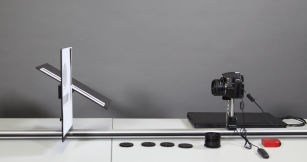
\includegraphics[width=0.7\textwidth]{bilder/aufbau.png}
		\caption{Darstellung des Versuchsaufbau. Dabei ist (1) das Spektrometer, (2) die Lichtquelle und (3) ein Prisma.\cite{WWU}}
		\label{fig:aufbau}	
	\end{figure}	
	Der grundlegende Aufbau ist in Abb. \ref{fig:aufbau} dargestellt und für alle Teilversuche gleich.
	Dabei ist (1) das Spektrometer, (2) die Lichtquelle und (3) ein Prisma.
	Die Lichtquelle soll so auf das Spektrometer gerichtet werden, dass das Licht durch eine Spaltblende an dem einem Arm des Spektrometers verläuft und auf das Prisma trifft.
	An dem anderem Arm befindet sich ein Okular mit einem Fadenkreuz, sodass die erkennbaren Spektrallinien eingeordnet werden können.
	Dazu dient eine Gradskala auf dem Spektrometer.
	An dieser lässt sich der Winkel ablesen bei dem das Fadenkreuz in dem Okular liegt.
	
	Als erstes soll eine Natriumdampflampe als Lichtquelle verwendet werden und das Prisma so in den Strahlengang gebracht werden, dass dieser symmetrisch durch das Prisma geht.
	Darauf soll das Linienspektrum von Natrium hinter dem Okular betrachtet und die Beobachtungen erläutert werden.
	Anschließend soll mit einem 300-Spalt-pro-\si{\milli\meter} Transmissionsgitter statt des Prismas das Linienspektrum betrachtet werden.
	Analog dazu danach mit einem Gitter mit doppelt so vielen Spalte pro \si{\milli\meter}.
	Für die drei verschiedenen dispergierenden Elemente soll das Auflösungsvermögen anhand der Beugungsordnungen und der Na $D$-Linie diskutiert werden.
	
	Bei dem zweitem Teilversuch soll zur Bestimmung des Gases in einer Energiesparlampe zunächst das Linienspektrum einer Heliumlampe herangezogen werden.
	Hier soll weiterhin das 600-Spalt-pro-\si{\milli\meter} Transmissionsgitter verwendet werden.
	Eine Tabelle der Wellenlängen die den einzelnen Spektrallinien zugehören ist für diesen Versuch gegeben.
	Mit Hilfe der Tabelle, des Fadenkreuzes an dem Okular und der Gradskala soll eine Funktion für die Wellenlänge in Abhängigkeit des Winkels durch diese Spektrallinien erstellt werden.
	Daraufhin soll das Linienspektrum der Energiesparlampe betrachtet werden und anhand der Wellenlängen, die sich aus der aufgestellten Funktion ergeben, das Gas identifiziert werden mit dem die Lampe gefüllt ist.
	
	Für den letzten Teilversuch sollen die Spektren verschiedenfarbiger Leuchtdioden betrachtet werden.
	Dazu sollen die Wellenlänge des Emissionsmaximum bestimmt werden.
	Auch hier soll die Beobachtung mit dem 600-Spalt-pro-\si{\milli\meter} Transmissionsgitter durchgeführt werden.
	Zudem soll für jede der Dioden die Spannung gemessen werden, ab der sie zu leuchten beginnen.
	Zuletzt sollen die zugehörigen Spannungen als Funktionswerte des Kehrwerts der entsprechenden Wellenlänge aufgetragen werden und $hc$ daraus bestimmt werden.
	
\section{Durchführung}
		
	Da andere Gruppen den Versuch bereits zuvor an dem selben Spektrometer durchgeführt hatten, war die Justierung des Spektrometers bereits erledigt, wurde jedoch vor Beginn der Messung überprüft.
	
	Die Durchführung erfolgte analog zu der Beschreibung in Abschnitt \ref{sec:Methoden}.
	Hierbei traten keine unerwarteten Effekte auf.
	
	Für die Natriumdampflampe ließ sich nur eine breite gelbe Spektrallinie und einige weitere schwächere beobachten (darunter eine blaue, eine türkisfarbene, eine grüne und eine rote).
	Bei den Gittern hingegen ließen sich ab den dritten Beugungsmaxima jedoch schon zwei gelbe Linien, welche sehr nah aneinander lagen erkennen.
	Der Abstand zwischen diesen wurde mit höheren Beugungsmaxima größer.
	Mehr als vier Maxima pro Seite ließen sich nicht beobachten.
	
	Die Winkel der beiden gelben Natriumlinien, sowie der für das Helium- und Energiesparlampenlinienspektrum sind dem Laborbuch zu entnehmen.
	
	Bei den Leuchtdioden wurden jeweils eine rote, gelbe, grüne und blaue verwendet.
	Das nullte Maximum entsprach bei allen Dioden einer Linie in ihrer Farbe.
	Die ersten Maxima hingegen waren für alle Dioden wie verschmierte Bänder und einzelne Maxima waren nur schwer zu erkennen.
	Alle Bänder besaßen einen Farbverlauf, welcher einen Teil des Gesamtspektrums ausmachte.
	Bei der roten Leuchtdiode war das Band nahezu komplett rötlich, das der gelben jedoch hatte bereits eine kontinuierliche Verteilung von grün bis rot.
	Für die grüne Leuchtdioden traten die Farben von türkis bis rot auf und bei der blauen alle von violett bis rot.
	Die Intensität war bei letzteren drei bei ihrer eigenen Farbe (gelb, grün bzw. blau) am höchsten.
	Vor Betrachtung der Linienspektren wurde für jede der Dioden die Einsatzspannung drei mal gemessen, da die Unsicherheit für eine einzelne Messung zu groß wäre.
	Bei diesen fällt auf, dass die Einsatzspannungen der Dioden mit Anteilen geringerer Wellenlängen höher liegen als andere.   
		
\section{Datenanalyse} \label{sec:Analyse}
	
	\begin{figure}[ht]
		\centering
		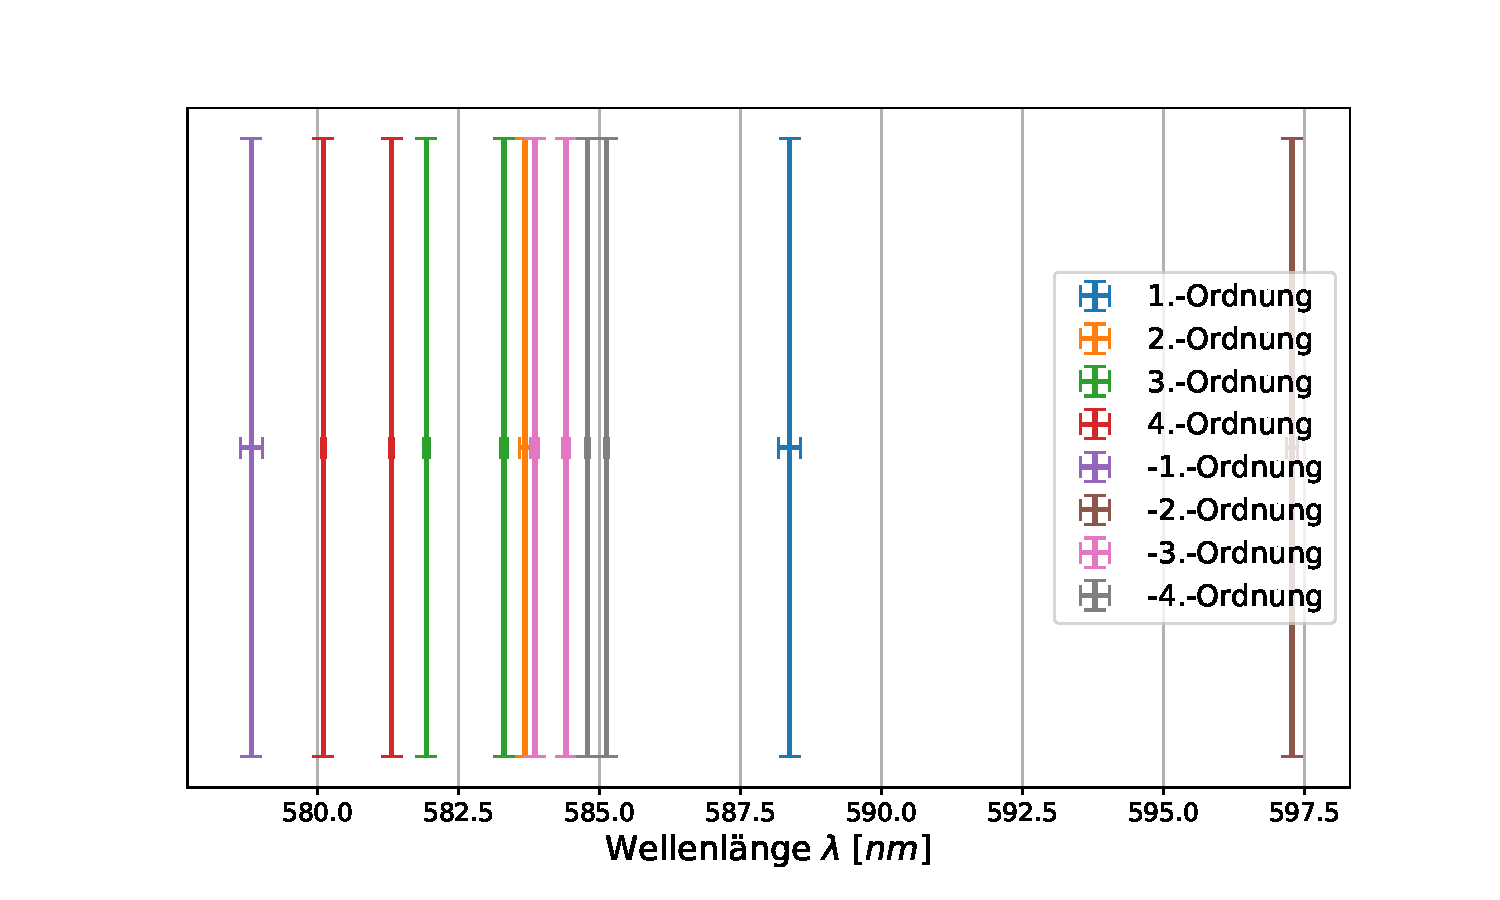
\includegraphics[width=\textwidth]{data/Gitter300.pdf}
		\caption{Spektrallinien der Beugungsmaxima der Na $D$-Linie bei dem 300-Spalt-pro-\si{\milli\meter} Transmissionsgitter.}
		\label{fig:Gitter300}	
	\end{figure}
	\begin{figure}[ht]
		\centering
		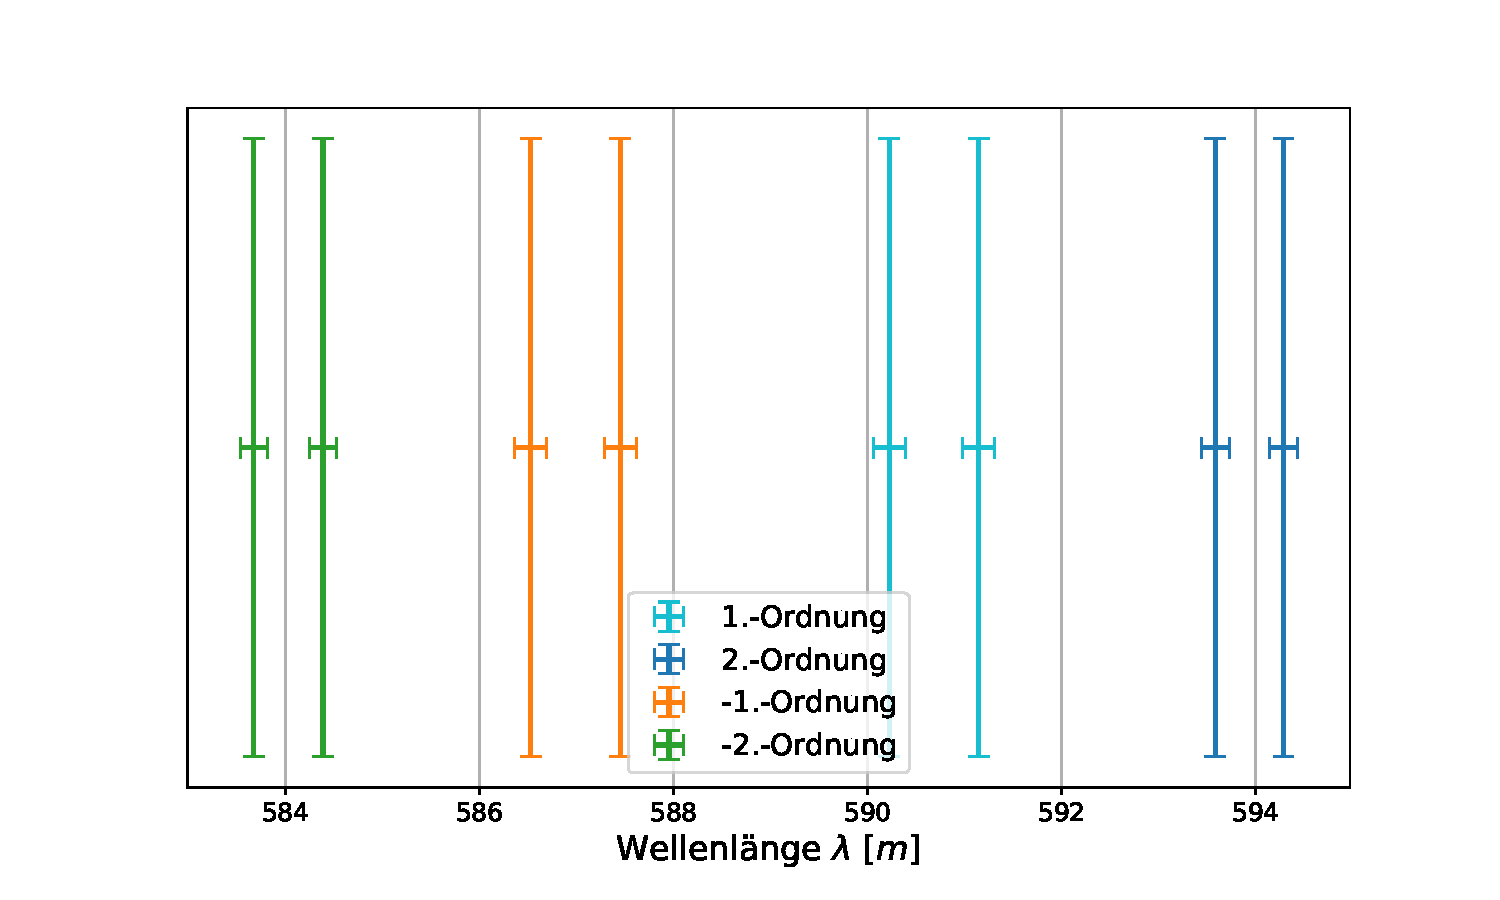
\includegraphics[width=\textwidth]{data/Gitter600.pdf}
		\caption{Spektrallinien der Beugungsmaxima der Na $D$-Linie bei dem 600-Spalt-pro-\si{\milli\meter} Transmissionsgitter.}
		\label{fig:Gitter600}	
	\end{figure}
	Aus den gemessenen Winkeln der verschiedenen Beugungsmaxima für die Na $D$-Linie wurden die zugehörigen Wellenlängen bestimmt.
	Diese sind für das erste Gitter in Abb. \ref{fig:Gitter300} und für das zweite Gitter in Abb. \ref{fig:Gitter600} aufgetragen.
	Dabei gehören zwei gleichfarbige Linien zu der gleichen Ordnung.
	Ist nur eine zu erkennen, so liegen beide aufeinander.
	Die zugehörigen Wellenlängen ergaben sich aus Gleichung \ref{eq:linear}.
	Auffällig ist, dass diese voneinander abweichen, obwohl es sich um nur zwei Wellenlängen für alle Ordnungen handeln sollte.
	
	Nun zu dem Linienspektrum des Heliums.
	Da nicht alle Spektrallinien aus der Tabelle den beobachteten zuzuordnen waren wurden, wurden nicht alle zu der Aufstellung einer Funktion der Wellenlänge verwendet.
	\begin{figure}[ht]
		\centering
		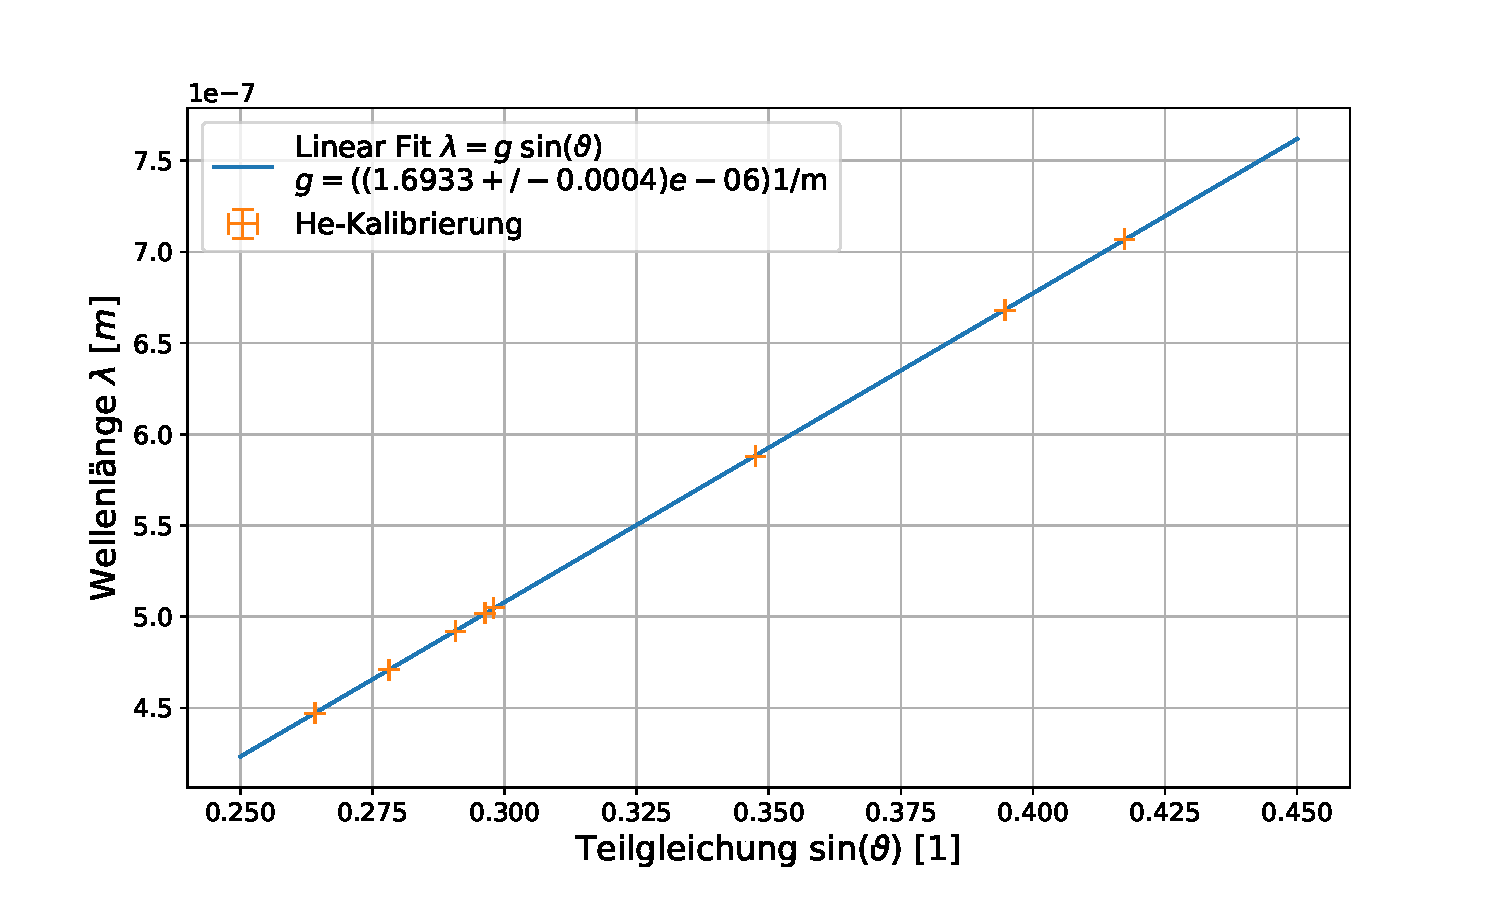
\includegraphics[width=\textwidth]{data/GitterConstPruef.pdf}
		\caption{Darstellung der Wellenlänge in Abhängigkeit des Sinus des gemessenen Winkels für die Heliumlampe mit linearerem Fit.}
		\label{fig:Funktion}	
	\end{figure}
	Abbildung \ref{fig:Funktion} stellt den Zusammenhang zwischen den gemessenen Winkeln der Spektrallinien und dazu zugehörigen Wellenlängen dar.
	Damit ein linearer Fit verwendet werden konnte wurde der Sinus der Winkel aufgetragen.
	Das lineare Verhältnis folgt aus:
	\begin{equation} \label{eq:linear}
		\Delta\lambda = \Delta\sin{\vartheta_m} \frac{g}{m},
	\end{equation}
	wobei $m$ die Zahl des Beugungsmaximums	und $g$ die Gitterkonstante ist.
	\begin{figure}[ht]
		\centering
		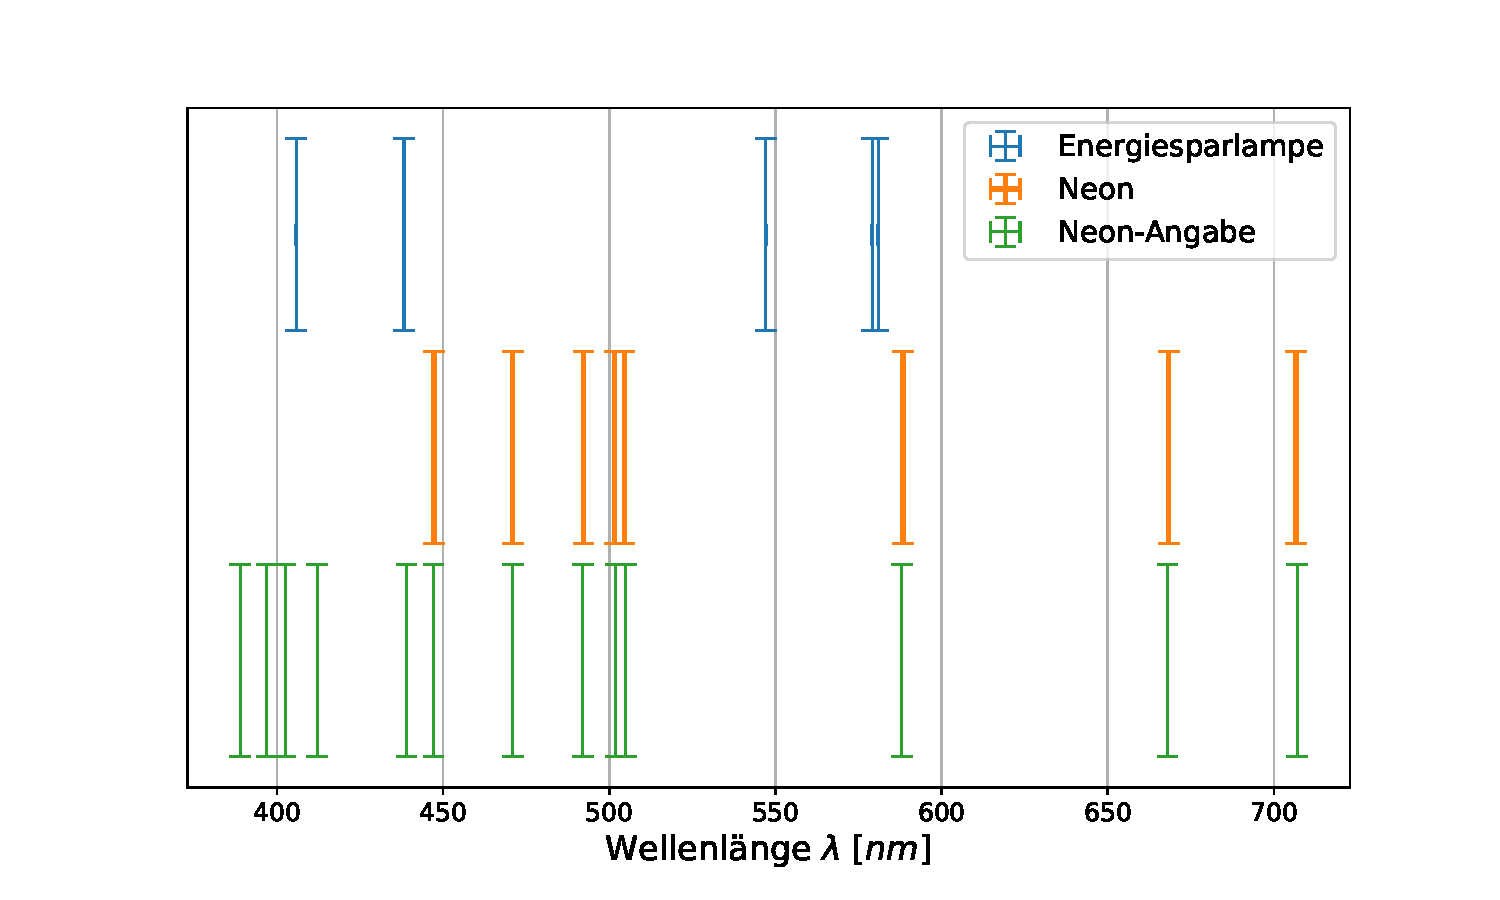
\includegraphics[width=\textwidth]{data/EnergieSpar.pdf}
		\caption{Darstellung der Spektrallinien der Werte für Helium aus der Tabelle (grün), der gemessenen für Helium (orange) und der gemessenen der Energiesparlampe (blau).}
		\label{fig:Linien}	
	\end{figure}
	Hiermit und mit den Winkeln für die Energiesparlampe ergaben sich die Ergebnisse in Abb. \ref{fig:Linien}.
	Die fünf erkennbaren Linien für die Lampe liegen bei \SI{405.81+-0.13}{\nano\meter}, \SI{438.25+-0.14}{\nano\meter}, \SI{547.08+-0.16}{\nano\meter}, \SI{579.13+-0.16}{\nano\meter} und \SI{580.98+-0.16}{\nano\meter}.
	
	\begin{figure}[ht]
		\centering
		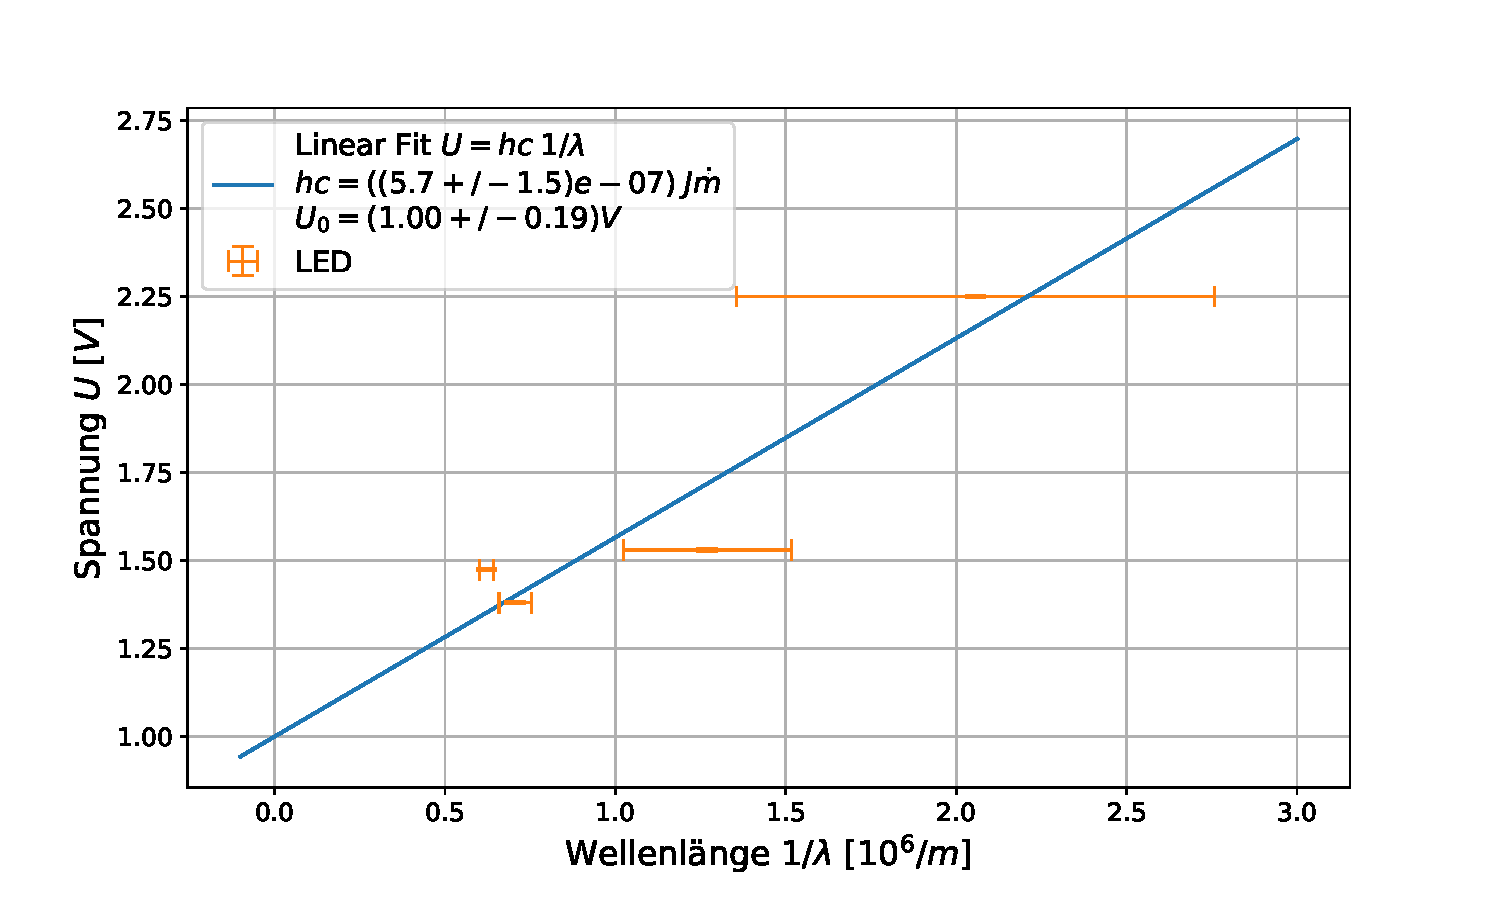
\includegraphics[width=\textwidth]{data/Dioden.pdf}
		\caption{Darstellung der Einsatzspannung für die vier verschiedenen Wellenlängen, bei denen die Intensitätsmaxima der einzelnen Dioden liegen. Zudem linearer Fit um $hc$ zu bestimmen.}
		\label{fig:Dioden}	
	\end{figure}
	Bei dem letzten Teilversuch mit den Dioden ergab sich durch auftragen der gemittelten Spannungswerte der in Abb. \ref{fig:Dioden} dargestellte Verhalt.\footnote{Der Winkel für das Intensitätsmaximum bei der roten Leuchtdiode wurde nicht dokumentiert. Aufgrund dessen wurde der Winkel \SI{21,6}{\degree}\cite{Mo14} von Gruppe Mo14 für den linearen Fit verwendet.} 
	Aus $E = h\nu = hc / \lambda = eU$ folgt dass die Steigung bei dem Auftragen der Spannung $U$ gegen den Kehrwert der Wellenlänge $1/\lambda$ gerade $hc / e$ entspricht.
	Da die Wellenlänge, wie auch die Einsatzspannungen große Unsicherheiten besitzen, ist der lineare Fit und somit die Steigung ungenau.
	Es lässt sich der Steigung des linearen Fits folgern, dass $hc = \SI{5,7+-1,5e-7}{\electronvolt\meter}$ entspricht. 
			
\section{Diskussion}
	
	Zunächst rückblickend die Behauptungen von Studentengruppe A: Die gelbe Natrium $D$-Linie lässt sich nicht in seine beiden Wellenlängen aufspalten. Bei der Energiesparlampe handelt es sich um eine mit Quecksilber befüllte. 
	Leuchtdioden besitzen jeweils nur eine Wellenlänge, da sie bestimmte Farben besitzen.
	Zudem lässt sich aus diesen einzelnen Wellenlängen die Proportionalität $hc$ zwischen $\Delta E$ und $\lambda^{-1}$ berechnen.
	
	Die Beobachtungen bei der Natriumdampflampe stimmen nicht mit der Behauptung überein.
	Bei dem Prisma war zwar keine Unterscheidung der Na $D$-Linie möglich, bei den Gittern ab dem dritten Beugungsmaximum jedoch schon.
	Hier war die Auflösung also groß genug um beide Linien zu erkennen.
	Dass die Spektrallinien in Abb. \ref{fig:Gitter600} nicht mit den Beobachtungen übereinstimmen deutet auf einen Fehler in der Berechnung oder der Aufnahme der Winkel hin.
	Zudem liegen bei dieser und Abbildung \ref{fig:Gitter300} die Wellenlängen für die Spektrallinien verstreut und nicht auf den beiden bei \SI{588.995}{\nano\meter} oder \SI{589.592}{\nano\meter}\cite{NISTNa}.
	So lässt sich an dieser Stelle keine genaue Aussage über die Wellenlängen der Na $D$-Linie treffen, die Behauptung von Studentengruppe A aufgrund der Beobachtungen dennoch widerlegen.
	
	Dass es sich bei dem Gas in der Energiesparlampe um Quecksilber handelt lässt sich bestätigen.
	Alle der Werte \SI{405.81+-0.13}{\nano\meter}, \SI{438.25+-0.14}{\nano\meter}, \SI{547.08+-0.16}{\nano\meter}, \SI{579.13+-0.16}{\nano\meter} und \SI{580.98+-0.16}{\nano\meter} liegen ca. \SI{0+-1}{\nano\meter} um die Literaturwerte\cite{NISTHg}.
	Insbesondere der dominanten Spektrallinien von Quecksilber bei \SI{404.656}{\nano\meter}\cite{NISTHg} verglichen mit \SI{405.81+-0.13}{\nano\meter} oder \SI{546.074}{\nano\meter}\cite{NISTHg} mit \SI{547.08+-0.16}{\nano\meter}.
	Die Ergebnisse stimmen demnach mit diesem Teil der Behauptung überein.
	
	Bei den Dioden sind die Ergebnisse wie auch bei der Natriumdampflampe nicht einfach in den Kontext einzuordnen.
	Aufgrund der Beobachtungen, dass das Linienspektrum bandförmig ist, lässt sich zumindest die Behauptung von Studentengruppe A widerlegen.
	Dass sich $hc$ auf \SI{5,7+-1,5e-7}{\electronvolt\meter} beläuft entspricht jedoch nicht der Erwartung, dass $hc = \SI{4.135e-15}{\electronvolt\second} \cdot \SI{2,998e8}{\meter\per\second} \approx \SI{1,240e-6}{\electronvolt\meter}$\cite{NIST}, welcher ungefähr doppelt so groß ist wie der berechnete Wert.
	Auch hier ist ein Fehler in der Messung oder bei der Berechnung nicht auszuschließen.
	Da das erkennen der Maxima in den Spektralbänder schwer fiel ist dies nicht unwahrscheinlich.
	Auch der Wert für das Maximum der roten Leuchtdiode, welches von einer anderen Gruppe stammt, könnte aufgrund unterschiedlicher Kalibrierung mit der Heliumlampe nicht genau in die Messung dieser Untersuchung passen.
	
	Somit lassen sich die Behauptungen der Studentengruppe A bis auf den Inhalt der Energiesparlampe und der Berechnung von $hc$ widerlegen.
	Für letztere ist keine genaue Aussage zu treffen.